\documentclass [12pt]{fhnwreport}
\usepackage[ngerman]{babel}
\usepackage[T1]{fontenc}
\usepackage[utf8]{inputenc}
\usepackage{tikz}
\usetikzlibrary{arrows}
\usepackage{amsmath}
\usepackage{lmodern}
\usepackage[final]{pdfpages}
\usepackage{graphicx}
\usepackage{textcomp}
\usepackage{multirow}
\usepackage{todonotes}
\usepackage{pdfpages}
\bibliographystyle{IEEEtran}
\usepackage{cite}
\usepackage[nottoc,notlof,notlot,numbib]{tocbibind}
\setboolean{@twoside}{false} 
%\usepackage[nottoc, numbib]{tocbibind}

\graphicspath{{./graphics/}}
\title{%
  \textsc{Laborfähiger Photovoltaiksimulator}\\
  \textsc{Pflichtenheft v\_2}}
\author{%
  \textsc{Projekt 3 - Team 3}\\
  \textsc{Simon Sturm, Yanick Frei,
Claudius Jörg}}
\date{\textsc{Windisch, 22.10.2015}}

\begin{document}
\maketitle
%\begin{center}
%\Large Laborfähiger Photovoltaiksimulator\\
%Pflichtenheft\\
%\large Projekt 3 - Team 3\\
%Simon Sturm, Yanick Frei, Claudius Jörg\\
%Windisch, 08.10.2015
%\end{center}


\textbf{Lösungskonzept}
\begin{itemize}
	\item Das Gerät hat intern ein galvanisch getrenntes Schaltnetzteil mit einer Ausgangsspannung von 24VDC und 3.5A Ausgangsstorm. Ripple-Noise beträgt weniger als 0.5\%.
	\item Das Gerät kann mittels Hauptschalter ein- und ausgeschaltet werden.
	\item Für weitere in Serie geschaltete Simulationsgeräte wird eine Freilaufdiode (Schottky) am Ausgang über dem Kondensator angebracht, damit das Gerät im Seriebetrieb nicht durch Rückwärtsspeisung zerstört wird.
	\item Die Ausgangskennlinie wird mittels eines Abwärtswandlers verwirklicht.
	\item Der Abwärtswandler wird mittels Mikrocontroller geregelt:\\
	Falls Strom- und Spannungswerte nicht übereinstimmen passt der	MC die Spannung an, bis diese mit dem gewünschten Strom übereinstimmt (Wertetabelle).
	\item Der Mikrocontroller besitzt genügend Ein- und Ausgänge für Messung, Display, Bedienung und Ansteuerung des Abwärtswandlers. Der interne Speicher ist genügend gross für Programm sowie Wertetabelle.
  \item Spannungs- und Stromwerte sowie die momentane Bestrahlungsstärke werden auf einem 4-Zeiligen Display ausgegeben.
	\item Die Strommessung wird mittels eines Hallsensors realisiert, die Spannungsmessung mit einem Spannungsteiler.
	\item Das Gerät hat eine separate 5V Referenzspannung, welche für die Messung mit den AD-Wandlern verwendet wird.
	\item Die Bedienung des Gerätes erfolgt mit zwei Tastern (+/-), mit denen die Bestrahlungsstärke in Prozent-Schritten von 20 bis 100 Prozent eingestellt werden kann. Die Schrittgrösse beträgt 1\%, falls die Tasten länger als 2s gedrückt bleiben, steigt die Bestrahlstärke um 10\% pro Sekunde. Die eventuelle Verschmutzung oder Teildefekte werden ebenfalls mit Tastern aktiviert.
	\item Die einzelnen Teile der Schaltung werden mittels LTSpice IV simuliert.
\end{itemize}

\textbf{Softwarekonzept}
\begin{itemize}
\item Beim Programmstart:
	\begin{itemize}
	\item Look-Up-Table mit Strom- und Spannungswerten laden (siehe unten).
	\item Display initialisieren
	\item Taster initialisieren
	\item Analoge Eingänge initialisieren
	\item Die Startspannung wird auf 5 Volt festgelegt.
	\end{itemize}
\newpage
\item Andauernd wiederholen:
	\begin{itemize}
	\item Strom messen
	\item Spannung messen
	\item Displayanzeige aktualisieren
	\item Strom und Spannung in Look-Up-Table nachschlagen
	\item Falls Strom zu klein: Spannung erhöhen
	\item Falls Strom zu gross: Spannung verringern
	\item Kurzes Delay
	\end{itemize}
	
\item Beim Tasterdruck:
	\begin{itemize}
	\item Werte der Look-Up-Table entsprechend der Formel bearbeiten.
	\end{itemize}
	
\item Look-Up-Table:\\
In der Look-Up-Table sind für die entsprechenden Prozentwerte die zu den Stromwerten zugehörigen Spannungswerte hinterlegt.
\end{itemize}

\textbf{Hardwarekonzept}\\
\begin{center}
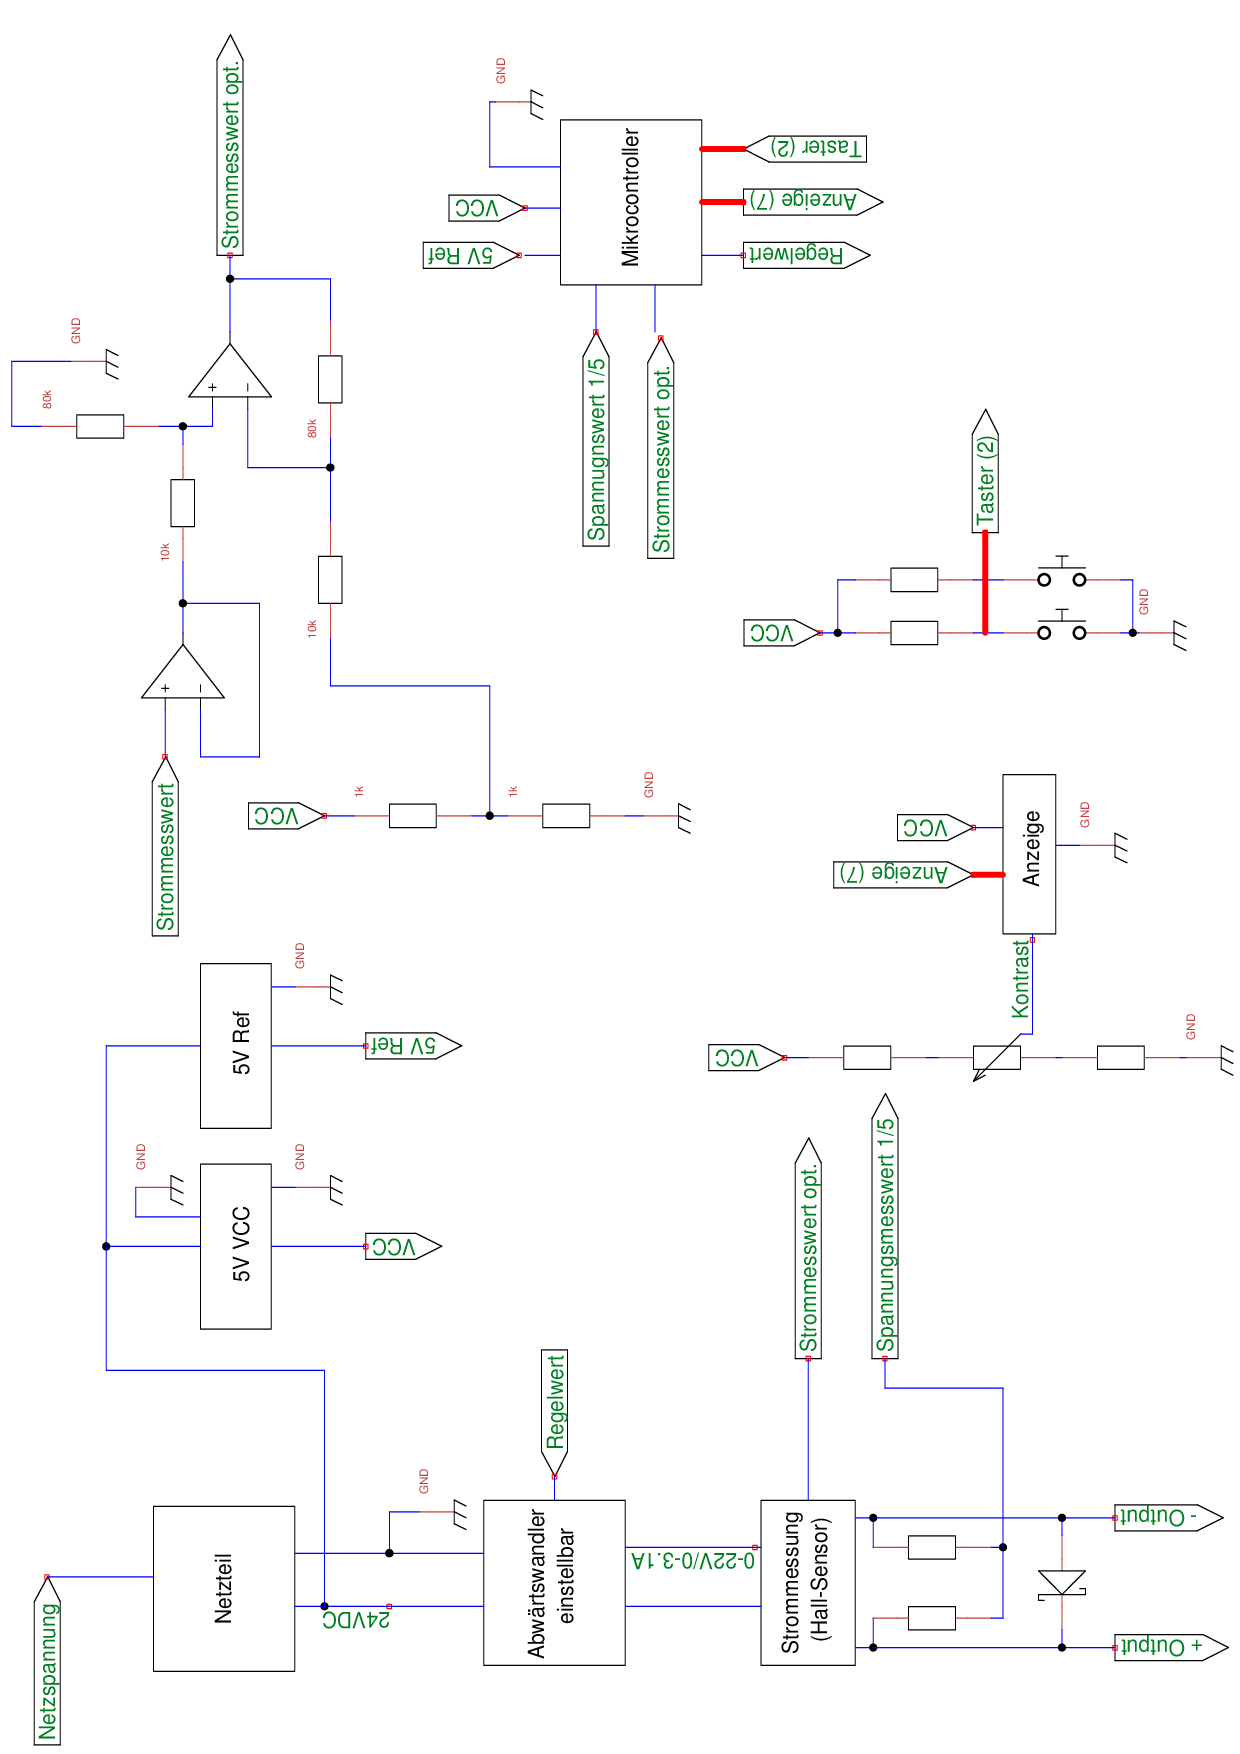
\includegraphics[angle=-90, width=0.8\textwidth]{Hardware_Prinzipschema.png}
\end{center}

\textbf{Testkonzept}
\begin{itemize}
	\item Die vorgängig notierten, zu erwarteten, Testwerte werden mit den Messergebnissen abgeglichen:
		\begin{itemize}
		\item Strom durch Stromwandler und entsprechende Ausgangsspannung am Stromwandler (185mV/A+2.5V Offset)
		\item Wert an OP Ausgang der Strommessung: (1.25V/Ampere)
		\item Spannung an Spannungsteiler (0.2V/V) 
		\item Die Ausgangskennlinie des Gerätes wird  gemessen und mit derjenigen im Lastenheft verglichen
		\item Der Rippel von Strom und Spannung darf nicht mehr als 5\% betragen
		\item Der Wirkungsgrad bei 100\%, 60\% und 20\% wird gemessen und als Grafik dargestellt. Dieser darf nicht kleiner als 95\% sein
		\end{itemize}
		
	\item Alle Änderungen werden protokolliert, um den Lösungsweg nachvollziehbar gestalten zu können.
\end{itemize}

%\newpage
%\bibliography{literaturverzeichnis}
%\listoffigures
%\listoftables

\end{document}

